\subsection{Continuous Integration}
Continuous integration is a practice in software development to continuously combine all developers’ changes into the main repository several times per day, and run a set of predefined checks to ensure the changes made do not break existing functionality or pre-defined standards. 
\par
Doing so means each developer has a near-latest sane copy of the code before making changes allowing for a reduction in the effort expended in tracking defects between different commits  
\par
In doing continuous integration, code changes pushed to the main repository  trigger the CI system to execute the steps defined in the pipeline.
Such steps may include but are not limited to: building the different executables (main and test applications), running unit test suites, acceptance test suites, static analysers (code quality and style checkers) as well as any other defined gradle, shell or other scripts.  
\par
For this project, we setup several Jenkins pipelines which are triggered upon each commit of the code. There are many ways to trigger builds in Jenkins, one such way is to continuously poll the repository for changes. 
Another is to trigger the build manually using HTTP POST. In our test implementation we have written a script to trigger the build manually using curl, a linux tool. The script is run after every commit made. 
\begin{itemize}
    \item TaxCalc-build
	\item TaxCalc-test-acceptance
	\item TaxCalc-test-unit
\end{itemize}

\begin{figure}[H]
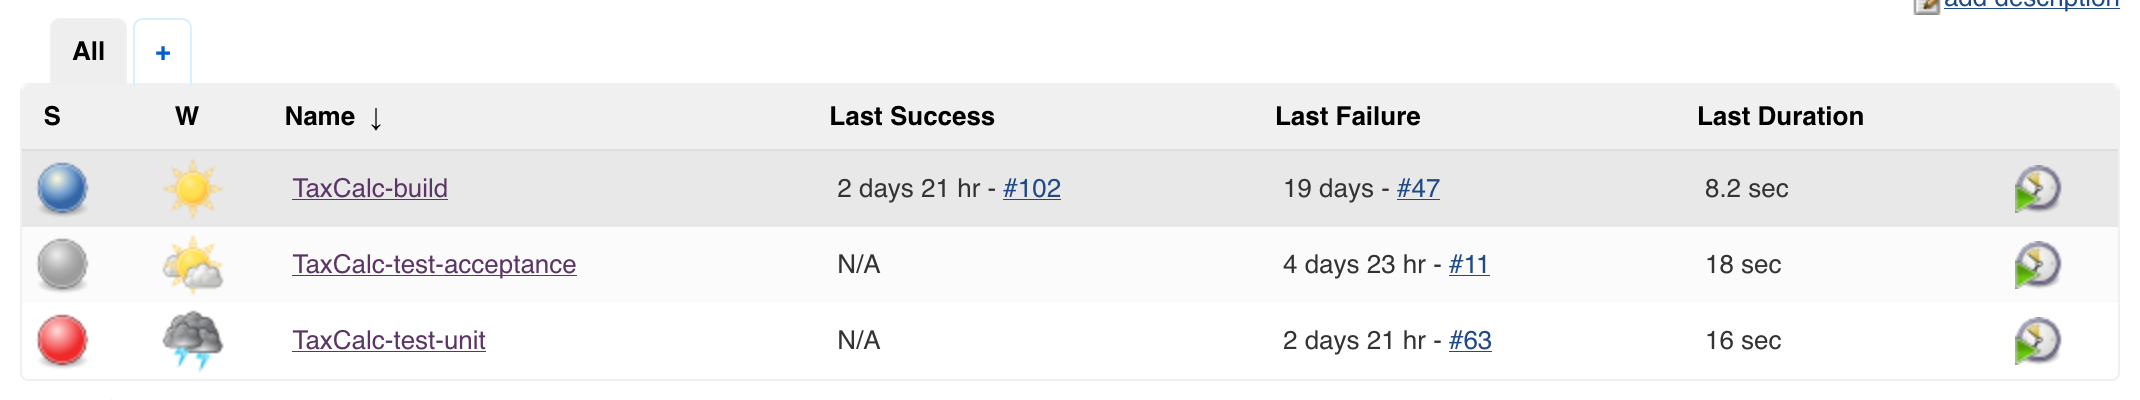
\includegraphics[scale=0.4]{res/jenkins.png}
\label{fig:jenkins-screenshot}
\caption{Screenshot: Jenkins Project}
\end{figure}